% Created 2024-04-20 Sat 11:07
% Intended LaTeX compiler: pdflatex
\documentclass[bigger]{beamer}
\usepackage[utf8]{inputenc}
\usepackage[T1]{fontenc}
\usepackage{graphicx}
\usepackage{longtable}
\usepackage{wrapfig}
\usepackage{rotating}
\usepackage[normalem]{ulem}
\usepackage{amsmath}
\usepackage{amssymb}
\usepackage{capt-of}
\usepackage{hyperref}
\usetheme{default}
\author{Alexander Brown}
\date{\today}
\title{A SIMULATED ANNEALING APPROACH TO THE BATTERY ELECTRIC BUS CHARGING PROBLEM}
\hypersetup{
 pdfauthor={Alexander Brown},
 pdftitle={A SIMULATED ANNEALING APPROACH TO THE BATTERY ELECTRIC BUS CHARGING PROBLEM},
 pdfkeywords={},
 pdfsubject={},
 pdfcreator={Emacs 29.3 (Org mode 9.6.15)}, 
 pdflang={English}}
\begin{document}

\maketitle
\begin{frame}{Outline}
\tableofcontents
\end{frame}


\section{Introduction}
\label{sec:orgb8562d0}
\begin{frame}[label={sec:orgca43c22}]{Problem Description}
\begin{columns}
\begin{column}{0.5\columnwidth}
\begin{itemize}
\item total of \(n_A\) buses in the fleet
\item \(n_V\) visits\footnote{A visit is when a bus arrives, receives a charge, and then departs} to the station divided between the \(n_A\) buses
\item Each bus in initialized with a charge of \(\alpha_b \kappa_i\)
\end{itemize}
\end{column}

\begin{column}{0.5\columnwidth}
\begin{itemize}
\item After each visit the bus goes on its route and discharges by \(\Delta_i\)
\item The charge is not allowed to go below \(\nu_b \kappa_i\) during operational hours
\item Each bus is required to finish the day with a minimum charge of \(\beta_b \kappa_i\)\footnote{PAP application only}
\end{itemize}
\end{column}
\end{columns}
\end{frame}

\begin{frame}[label={sec:orgf4f2cec}]{Mixed Integer Linear Programming}
\begin{subequations}
\label{eq:milp-structure}
\begin{align}
&\text{max}        &J = \sum_j c_j x_j + \sum_k d_k y_k&         &               &\label{eq:fuzzy-milp-objective}\\
&\text{subject to} &\sum_j a_{ij} x_j + \sum_k g_{ik} y_k \le b_i&  &(i = 1,2,...,m)& \label{eq:fuzzy-milp-constraint}\\
&                  &x_j \ge 0&                              &(j = 1,2,...,n)& \label{eq:fuzzy-milp-continuous}\\
&                  &y_k \in \mathbb{Z^+}&                   &(k = 1,2,...,n)& \label{eq:fuzzy-milp-integer}\\
&\end{align}
\end{subequations}

\begin{itemize}
\item \(J\): Objective function
\item \(x_j \in \mathbb{R}\) and \(y_k \in \mathbb{Z}^+\): Decision Variables
\item \(c_j, d_k, a_{ij}, g_{ik}, b_i \in \mathbb{R}\): Parameters
\end{itemize}
\end{frame}

\begin{frame}[label={sec:org20f3c86}]{The Berth Allocation Problem\footnote{\url{https://www.mdpi.com/2077-1312/11/7/1280}}}
The BAP solves the problem of optimally assigning incoming vessels to berth positions to be serviced

\begin{figure}[htpb]
\centering
    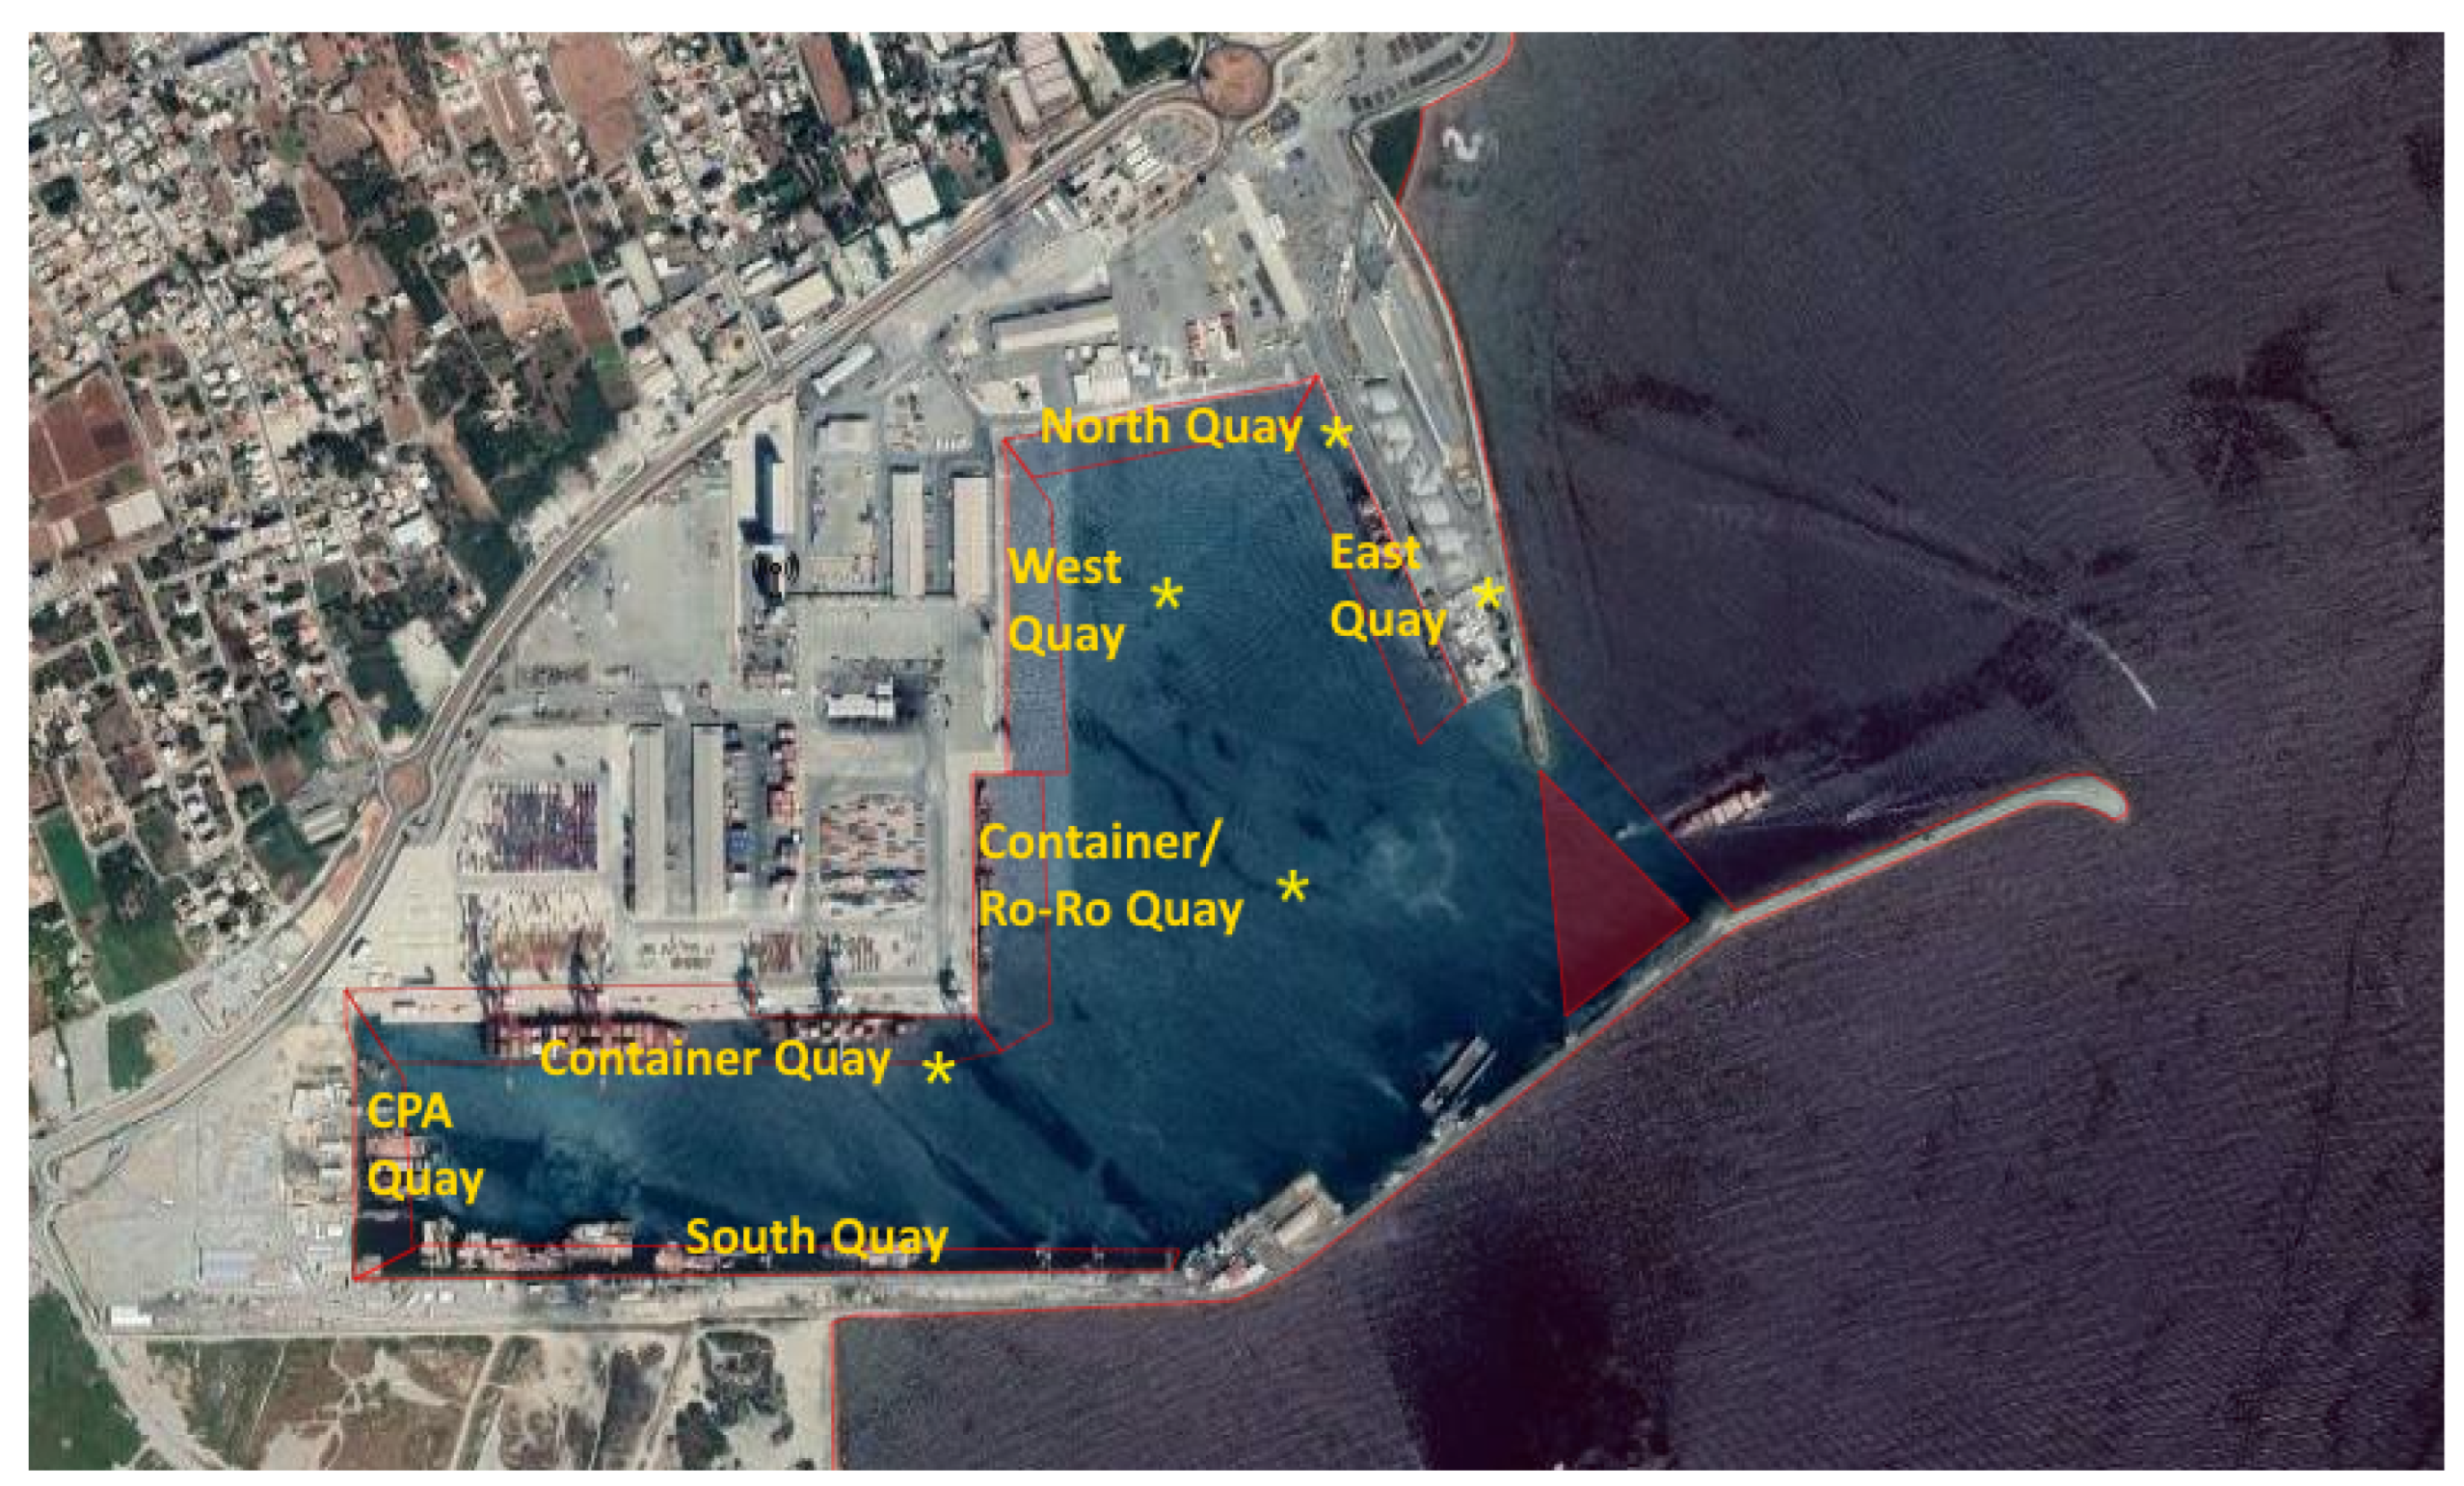
\includegraphics[width=0.9\textwidth]{img/berthing-sky-picture}
\end{figure}
\end{frame}

\begin{frame}[label={sec:orgaee3668}]{The Berth Allocation Problem}
The BAP is a variant of the rectangle packing problem

\begin{figure}[htpb]
\centering
    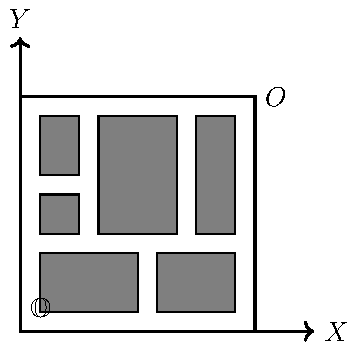
\includegraphics[width=0.5\textwidth]{img/spatiotemporal-packing}
\end{figure}
\end{frame}

\begin{frame}[label={sec:orgb5f7cd6}]{The Berth Allocation Problem}
\begin{columns}
\begin{column}{0.5\columnwidth}
\begin{itemize}
\item Vessels move down toward the quay
\item Recieve service
\item Exit to the right
\end{itemize}
\end{column}

\begin{column}{0.5\columnwidth}
\begin{figure}[htpb]
\centering
    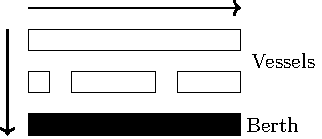
\includegraphics{img/bap}
    \label{subfig:bapexample}
\end{figure}
\end{column}
\end{columns}
\end{frame}


\begin{frame}[label={sec:org810cc46}]{The Position Allocation Problem}
\begin{columns}
\begin{column}{0.5\columnwidth}
\end{column}
\begin{column}{0.5\columnwidth}
\begin{figure}[htpb]
\centering
    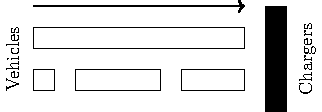
\includegraphics{img/pap}
    \label{subfig:papexample}
\end{figure}
\begin{itemize}
\item High level explanation
\item PAP assumptions
\end{itemize}
\end{column}
\end{columns}
\end{frame}
\section{The Position Allocation Problem Approach With Linear Battery Dynamic}
\label{sec:orgd798e25}
\begin{frame}[label={sec:org956b6d6}]{Introduction}
\begin{itemize}
\item What needs to change from the PAP
\item Contributions
\begin{itemize}
\item Charger minimization
\item Minimize consumption cost
\item BEB charge tracking
\end{itemize}
\end{itemize}
\end{frame}
\begin{frame}[label={sec:orga9e83bb}]{Objective Function}
\begin{itemize}
\item High level explanation
\end{itemize}
\end{frame}
\begin{frame}[label={sec:org389ed8e}]{Packing Constraints}
\begin{itemize}
\item High level explanation of how the constraints work
\end{itemize}
\end{frame}
\begin{frame}[label={sec:orga10b90b}]{Linear Battery Dynamic Constraints}
\begin{itemize}
\item High level explanation of how the constraints work
\end{itemize}
\end{frame}
\begin{frame}[label={sec:org1e8eeff}]{Results}
\begin{itemize}
\item How long it ran for
\item Plots!
\end{itemize}
\end{frame}
\section{The Simulated Annealing Approach With Linear Battery Dynamics}
\label{sec:org8bb97b5}
\begin{frame}[label={sec:org0d58bb9}]{Introduction}
\begin{itemize}
\item High level explanation
\begin{itemize}
\item Set of vessels
\item Schedule to place in berths to be serviced: image of berthing ships
\item Is essentially a rectangle packing problem: Example schedule plot
\end{itemize}
\end{itemize}
\end{frame}
\begin{frame}[label={sec:orgdab8638}]{Simulated Annealing}
\begin{itemize}
\item Basic introduction to what it is
\end{itemize}
\end{frame}
\begin{frame}[label={sec:orgd9a0677}]{Optimization Problem}
\begin{itemize}
\item Simplifications made
\item List constraints
\end{itemize}
\end{frame}
\begin{frame}[label={sec:org2f2c4e7}]{Algorithm}
\begin{itemize}
\item Outline components of the SA algorithm
\end{itemize}
\end{frame}
\begin{frame}[label={sec:org2ea4f73}]{Results - What Is In The Thesis}
\begin{itemize}
\item How long it ran for
\item It's sort of working, but not really
\end{itemize}
\end{frame}
\begin{frame}[label={sec:org6dd5a9c}]{What Happened?}
\begin{itemize}
\item Score Divergence
\item Difficult Schedules are\ldots{} difficult\ldots{}
\end{itemize}
\end{frame}
\begin{frame}[label={sec:org8518f48}]{How To Resolve This Problem?}
\begin{itemize}
\item Reverse search and weight the visit indices
\end{itemize}
\end{frame}
\begin{frame}[label={sec:org52c3f8c}]{Results - What Is Not In The Thesis}
\begin{itemize}
\item How long it ra for
\item Plots! WOW!
\end{itemize}
\end{frame}
\section{The Simulated Annealing Approach With Non-Linear Battery Dynamics}
\label{sec:org54657f3}
\begin{frame}[label={sec:org214a814}]{Introduction}
\begin{itemize}
\item Why even consider this?
\item Why use SA
\end{itemize}
\end{frame}
\begin{frame}[label={sec:org8b13bc8}]{Non-Linear Battery Dynamics Model}
\begin{itemize}
\item Show function
\item Show plots
\end{itemize}
\end{frame}
\begin{frame}[label={sec:orgf9b0797}]{Results}
\begin{itemize}
\item Figures!
\end{itemize}
\end{frame}
\end{document}
